\chapter{\IfLanguageName{dutch}{Stand van zaken}{State of the art}}
\label{ch:stand-van-zaken}

% Tip: Begin elk hoofdstuk met een paragraaf inleiding die beschrijft hoe
% dit hoofdstuk past binnen het geheel van de bachelorproef. Geef in het
% bijzonder aan wat de link is met het vorige en volgende hoofdstuk.

% Pas na deze inleidende paragraaf komt de eerste sectiehoofding.

In de inleiding is duidelijk geworden dat het onderzoek gericht zal zijn op twee mogelijke dataformaten aan de hand van 2 verschillende structuren, namelijk JSON aan de hand van REST en gRPC aan de hand van Protocol Buffers. Om dit onderzoek volledig te kunnen begrijpen is het belangrijk om de werking en de basisprincipes van deze dataformaten en de daarbij behorende structuren te begrijpen. Om deze reden zullen eerst de werking en basisprincipes van JSON en REST worden uitgelegd, en als volgt die van gRPC en Protocol Buffers.

\section{JSON}
\label{sec:JSON}

\subsection{Algemeen}
\label{subsec:Algemeen}

JavaScript Object Notation of in het kort, JSON, is zoals beschreven in Standard ECMA-404 ~\autocite{Json2017} een tekstsyntaxis of dataformaat dat geïnspireerd is door de object literalen van JavaScript dat ook gekend staat als ECMAScript. Het maakt een gegevensuitwisseling tussen alle programmeertalen op een gestructureerde manier mogelijk. Hiervoor maakt JSON gebruik van een structuur van accolades, haakjes, dubbele punten en komma's dewelke zeer nuttig kan zijn in verschillende contexten, profielen en applicaties. Ondanks dat JSON geïnspireerd is door ECMAScript probeert het de interne data representatie ervan niet op te leggen aan andere programmeertalen, in plaats daarvan deelt JSON een onderdeel van ECMAScript's syntax met alle andere programmeertalen. 

JSON mag niet gezien worden als een specificatie van een volledige gegevensuitwisseling want dat is het ook niet. Bij een zinvolle gegevensuitwisseling wordt er een overeenstemming over de semantiek die gekoppeld is aan een gebruik van de JSON-syntaxis tussen producent en consument vereist. JSON kan wel gezien worden als een syntactisch raamwerk waaraan een specifieke semantiek kan worden gekoppeld.

Doordat er veel verschillende types getallen zijn zoals, maar niet beperkt tot, decimale en binaire getallen, kiest JSON voor enkel een weergave van getallen die mensen gebruiken, namelijk een reeks cijfers. Ook al zijn alle programmeertalen het niet altijd eens over de interne representaties van getallen, ze weten wel hoe ze cijferreeksen moeten begrijpen.

Zoals nu wel duidelijk is kunnen programmeertalen sterk verschillen in mate van wat ondersteund wordt en hoe iets moet gerepresenteerd worden. Dit geldt ook voor objecten, niet alle programmeertalen ondersteunen objecten, en indien ze dit wel doen is er nog steeds een groot verschil in de kenmerken en beperkingen de objecten bieden. Met andere woorden kunnen de modellen van objectsystemen heel erg uiteenlopen. Om dit probleem aan te pakken biedt JSON een eenvoudige notatie aan voor het uitdrukken van verzamelingen met naam / waarde-paren. Om zulke verzamelingen weer te geven hebben de meeste programmeertalen reeds een functie zoals maar niet beperkt tot, struct, map, hash, object.
Daarnaast biedt JSON ook ondersteuning voor geordende zoeklijsten, alsook hiervoor hebben alle programmeertalen een functie om deze weer te geven zoals array, vector en list. Aangezien objecten en arrays zich kunnen nesten kunnen aan de hand van JSON complexe structuren zoals boomstructuren worden gerepresenteerd.

Hieruit kan dus geconcludeerd worden dat door het aanvaarden van JSON's simpele conventies, complexe datastructuren uitgewisseld kunnen worden tussen wat anders incompatibele programmeertalen zijn.



\subsection{Achterliggend}
\label{subsec:Achterliggend}

Een JSON-tekst bestaat uit een reeks tokens die gevormd zijn uit Unicode-codepunten en die in overeenstemming zijn met de JSON-waardegrammatica. Deze reeks tokens bevat tekenreeksen, cijfers, zes structurele token en drie letterlijke naamtokens.
Hieronder volgt een opsomming van de zes structurele tokens en de drie literal name tokens samen met de bijhorende Unicode.

De zes structurele tokens:

\begin{itemize}
    \item $\rbrack$ Linker vierkante haak, U+005B
    \item $\rbrack$ Rechter vierkante haak, U+005D
    \item \{ Linker accolade, U+007B
    \item \} Rechter accolade, U+007D
    \item : Dubbele punt, U+003A
    \item , Komma, U+002C
\end{itemize}

De drie literal name tokens:

\begin{itemize}
    \item true      U+0074 U+0072 U+0075 U+0065
    \item false     U+0066 U+0061 U+006C U+0073 U+0065
    \item null      U+006E U+0075 U+006C U+006C 
\end{itemize}

Voor of na een token is het toegestaan om onbelangrijke witruimte te gebruiken. Witruimte kan beschreven worden als een willekeurige reeks van één of meerdere van onderstaande codepunten.

\begin{itemize}
    \item Tekentabel        U+0009
    \item Regelinvoer       U+000A
    \item Regelterugloop    U+000D
    \item Spatie            U+0020
\end{itemize}

Witruimte is niet in elke token toegestaan, een spatie is hierop een uitzondering en is wel toegestaan in strings.

\subsection{Waarden}
\label{subsec:Waarden}

De bovengestelde tokens vormen de ruggengraad van een JSON-bestand, echter is het de bedoeling dat een JSON-bestaand iets van data overdraagd. Deze data kan aan de hand verschillende waarden worden voorgesteld, namelijk als objecten, arrays, nummers, strings, true, false, null.

\begin{figure}[h]
    \centering
    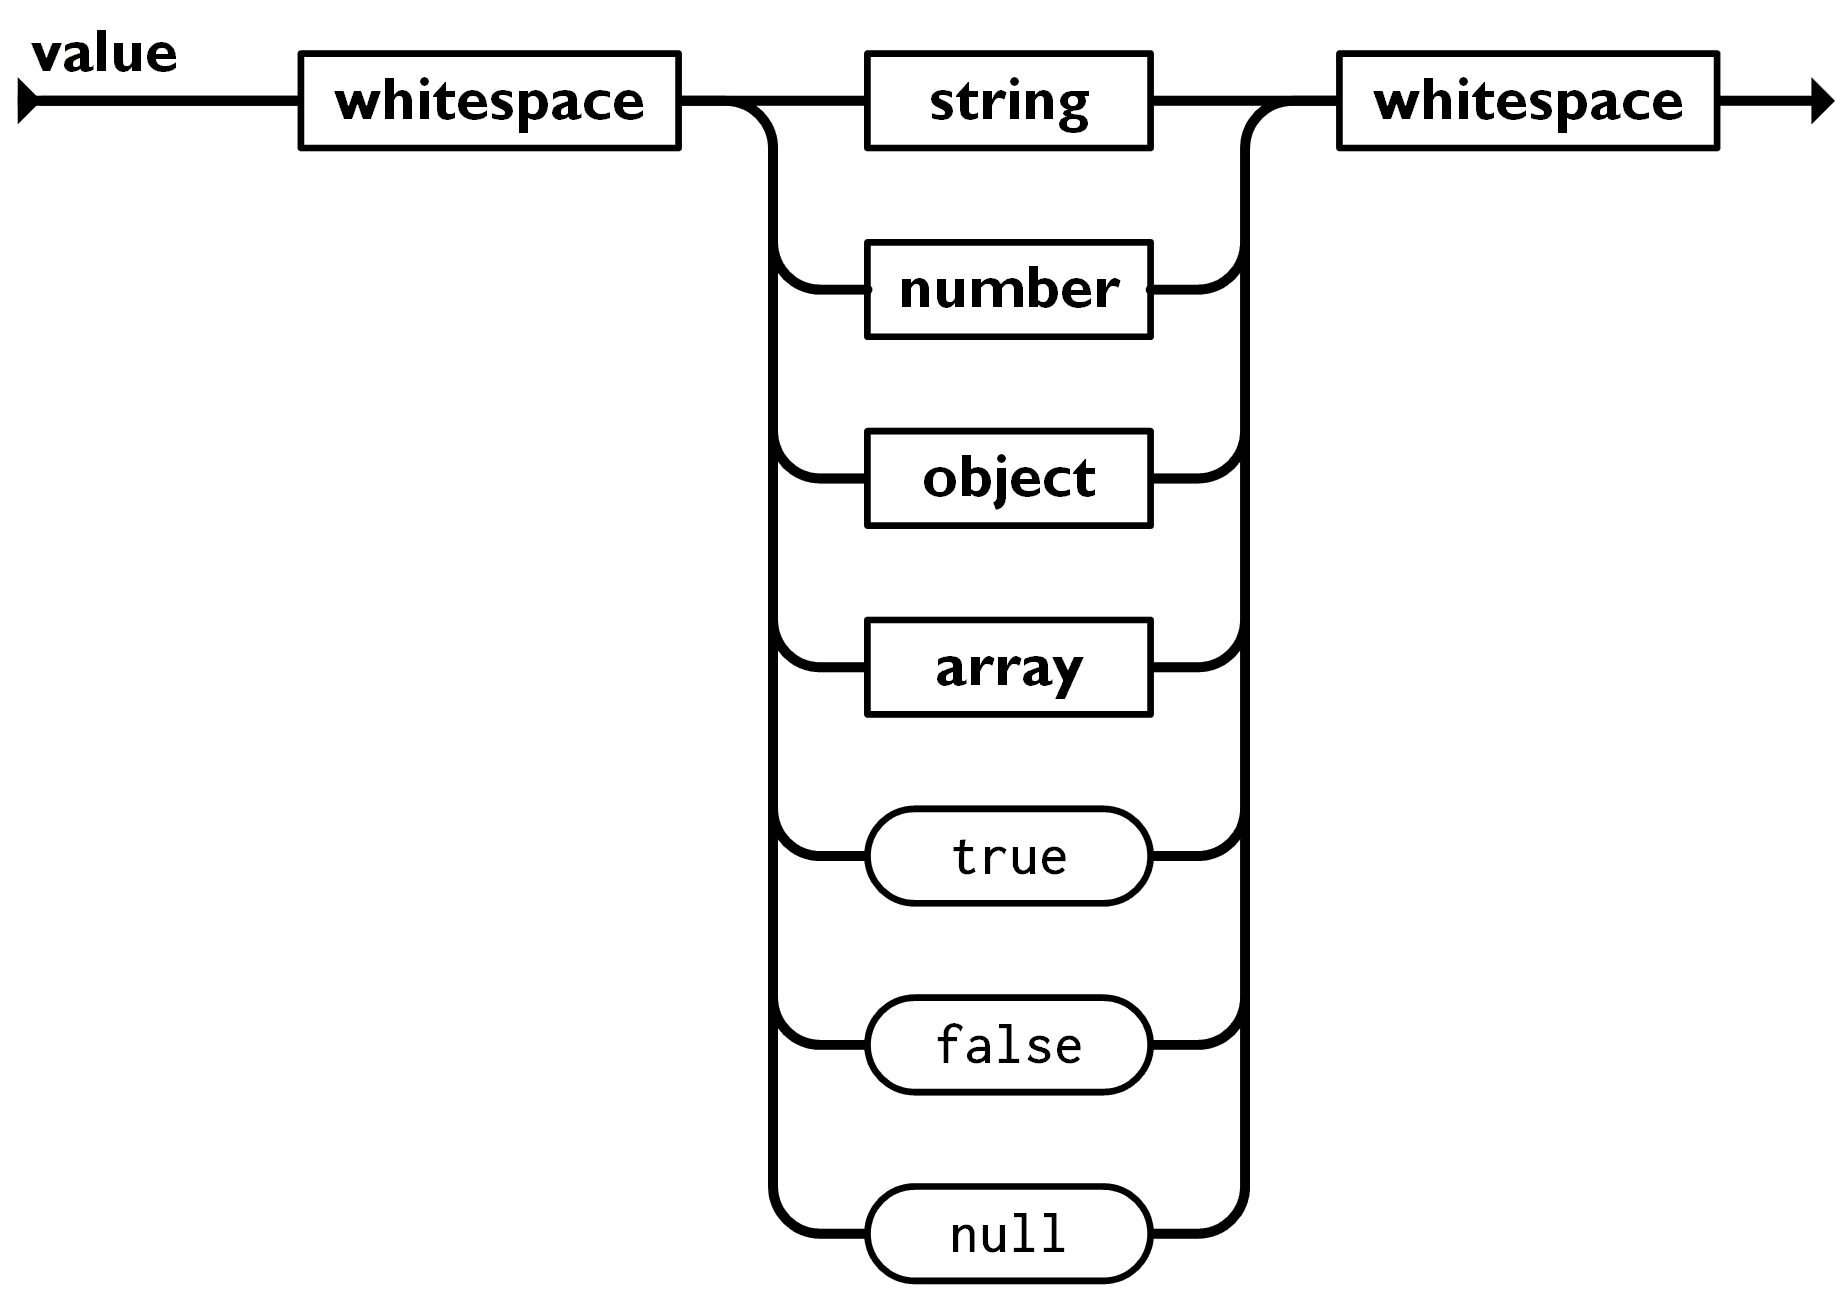
\includegraphics[scale=0.75]{jsonValue}
   \caption[JSON values]{De structuur van een JSON-waarde met alle mogelijke waarden die deze kan bevatten}
   \label{fig:jsonValue}
\end{figure}

De eerste waarden die besproken worden zijn de objecten, deze worden voorgesteld over een paar accolades die geen of meerdere name/value paren kunnen incapsuleren zoals te zien is in figuur \ref{fig:jsonObject}. In zo een name/value paar is de naam een string en wordt gevolgd door een dubbele punt die de naam en waarde van elkaar onderscheidt. Optioneel is een komma na de waarde, die de waarde en de eventuele volgende naam van elkaar onderscheiden. De JSON syntax legt geen beperkingen op op vlak van de strings gebruikt als namen. Deze moeten met andere woorden niet uniek zijn en ze moeten geen bepaalde ordening volgen.

\begin{figure}[h]
    \centering
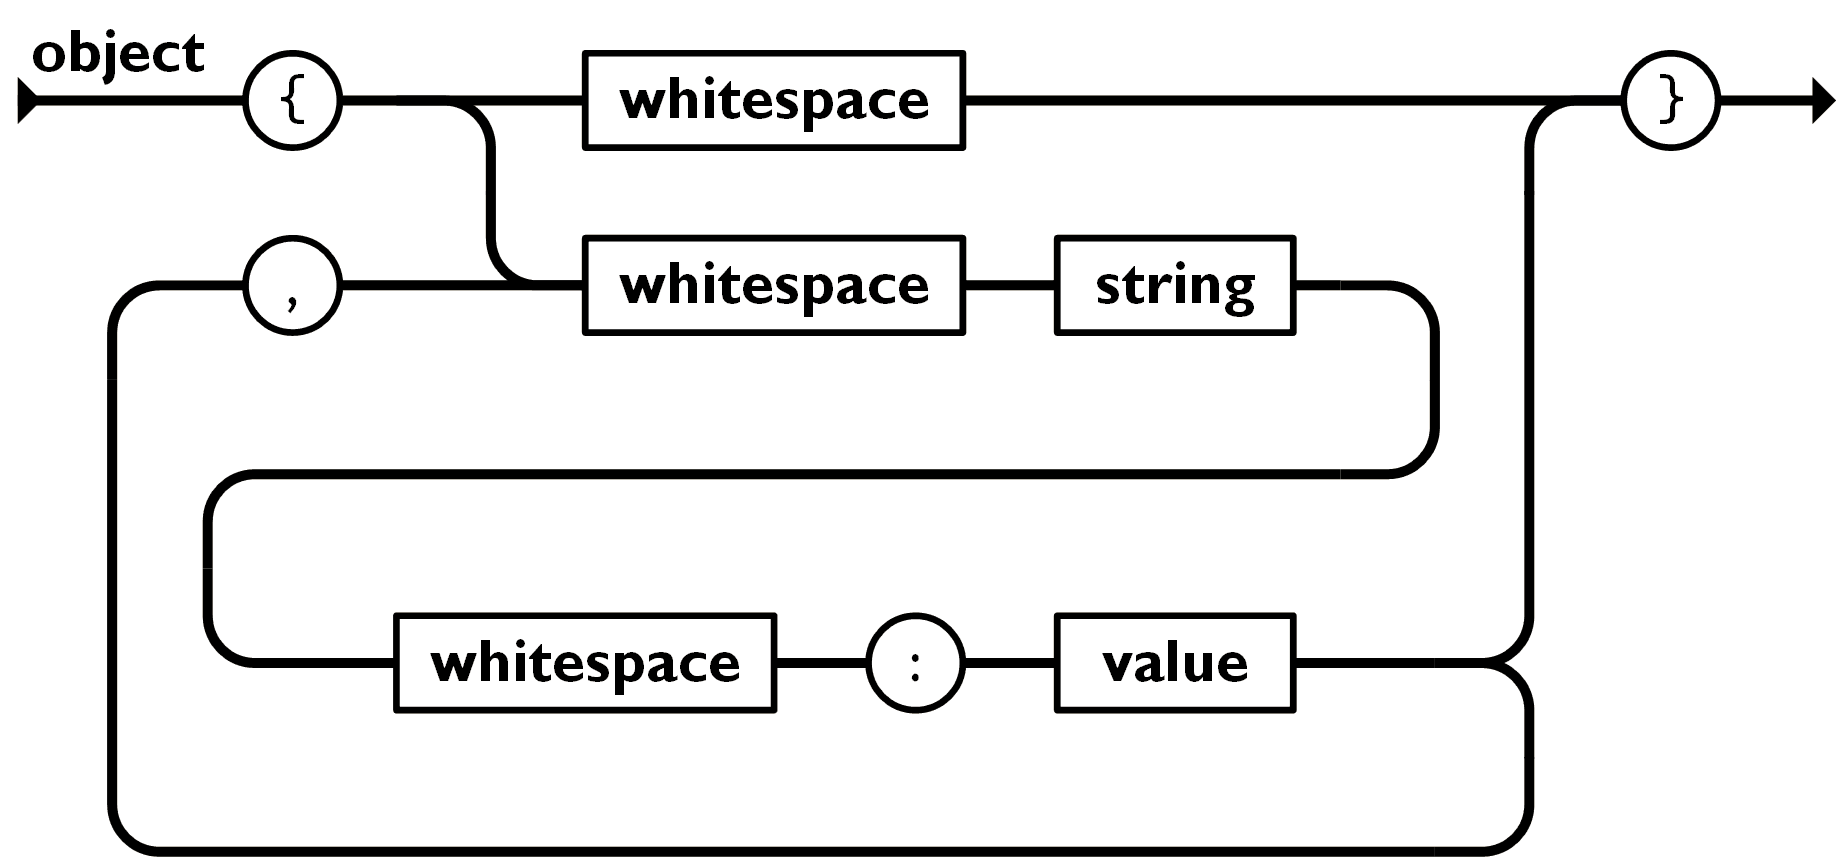
\includegraphics[scale=0.75]{jsonObject}
\caption[JSON Object]{De structuur van een JSON object.}
    \label{fig:jsonObject}
\end{figure}

Een tweede waarde zijn de arrays, dit zijn vierkante haken die geen of meerdere waarden incapsuleren. Het bijzondere aan arrays is dat deze niet beperkt zijn tot een name/value paar maar dat deze zelf dus meerdere waarden en dus ook andere arrays kunnen bevatten en dus genest kunnen worden. Dit kan afgeleid worden uit figuur \ref{fig:jsonArray}. De array structuur wordt net zoals bij objecten geen beperkingen opgelegd op vlak van de ordening van de waarden, echter wordt de array structuur vooral gebruikt in situaties waar de ordening wel enig belang heeft.

\begin{figure}[h]
    \centering
    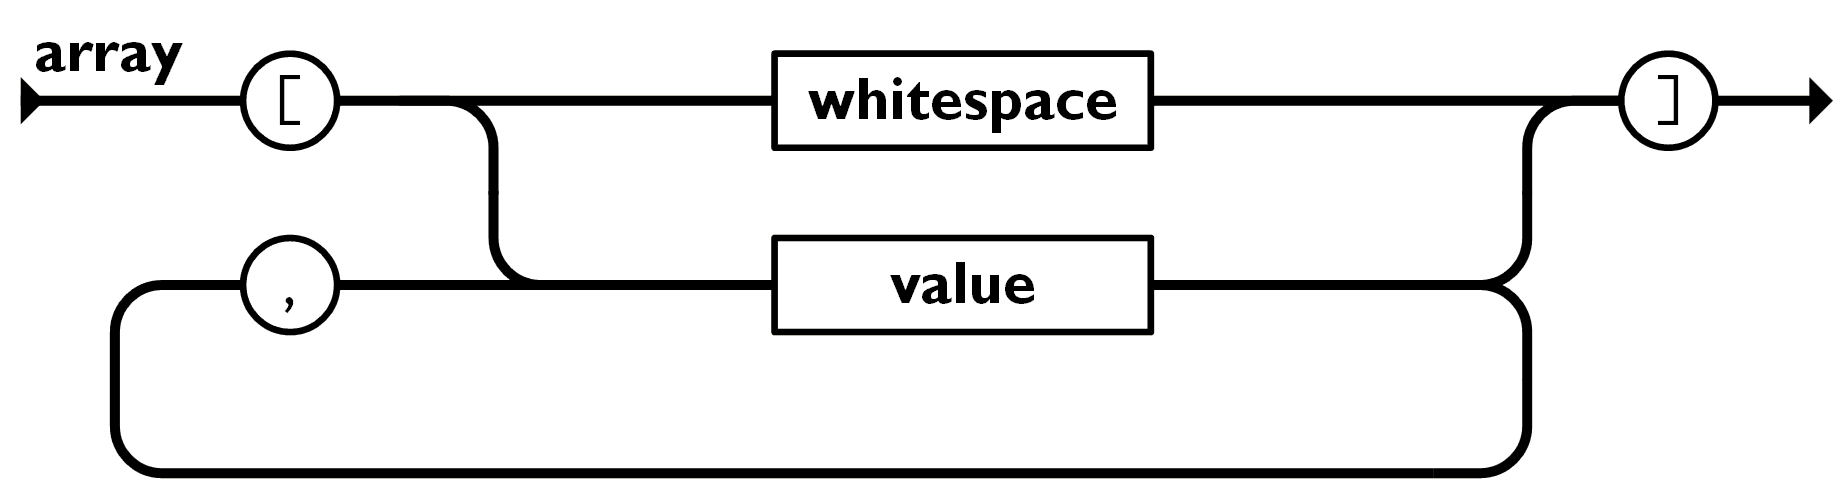
\includegraphics[scale=0.75]{jsonArray}
    \caption[JSON Array]{De structuur van een JSON array.}
    \label{fig:jsonArray}
\end{figure}

Als volgt zijn er de nummers, een nummer kan gedifinieerd worden als een sequentie van decimale cijfers. Bij deze sequentie cijfers is er geen overbodige voorloopnul, een nummer kan wel voorafgegaan worden door een min-teken met U+002D als Unicode code. Om te werken met kommagetallen wordt een decimaal punt gebruikt. Als ook kan een nummer voorafgegaan worden door een e met U+0065 als Unicode code of een E met U+0045 als Unicode code om een exponent aan te duiden, deze kunnen eventueel ook bijgestaan worden door + (U+002B) of - . Deze structuur is te zien in figuur \ref{fig:jsonNumber}.
In Unicode kunnen de cijfers gevonden worden van U+0030 tot en met U+0039. 

\begin{figure}[h]
    \centering
    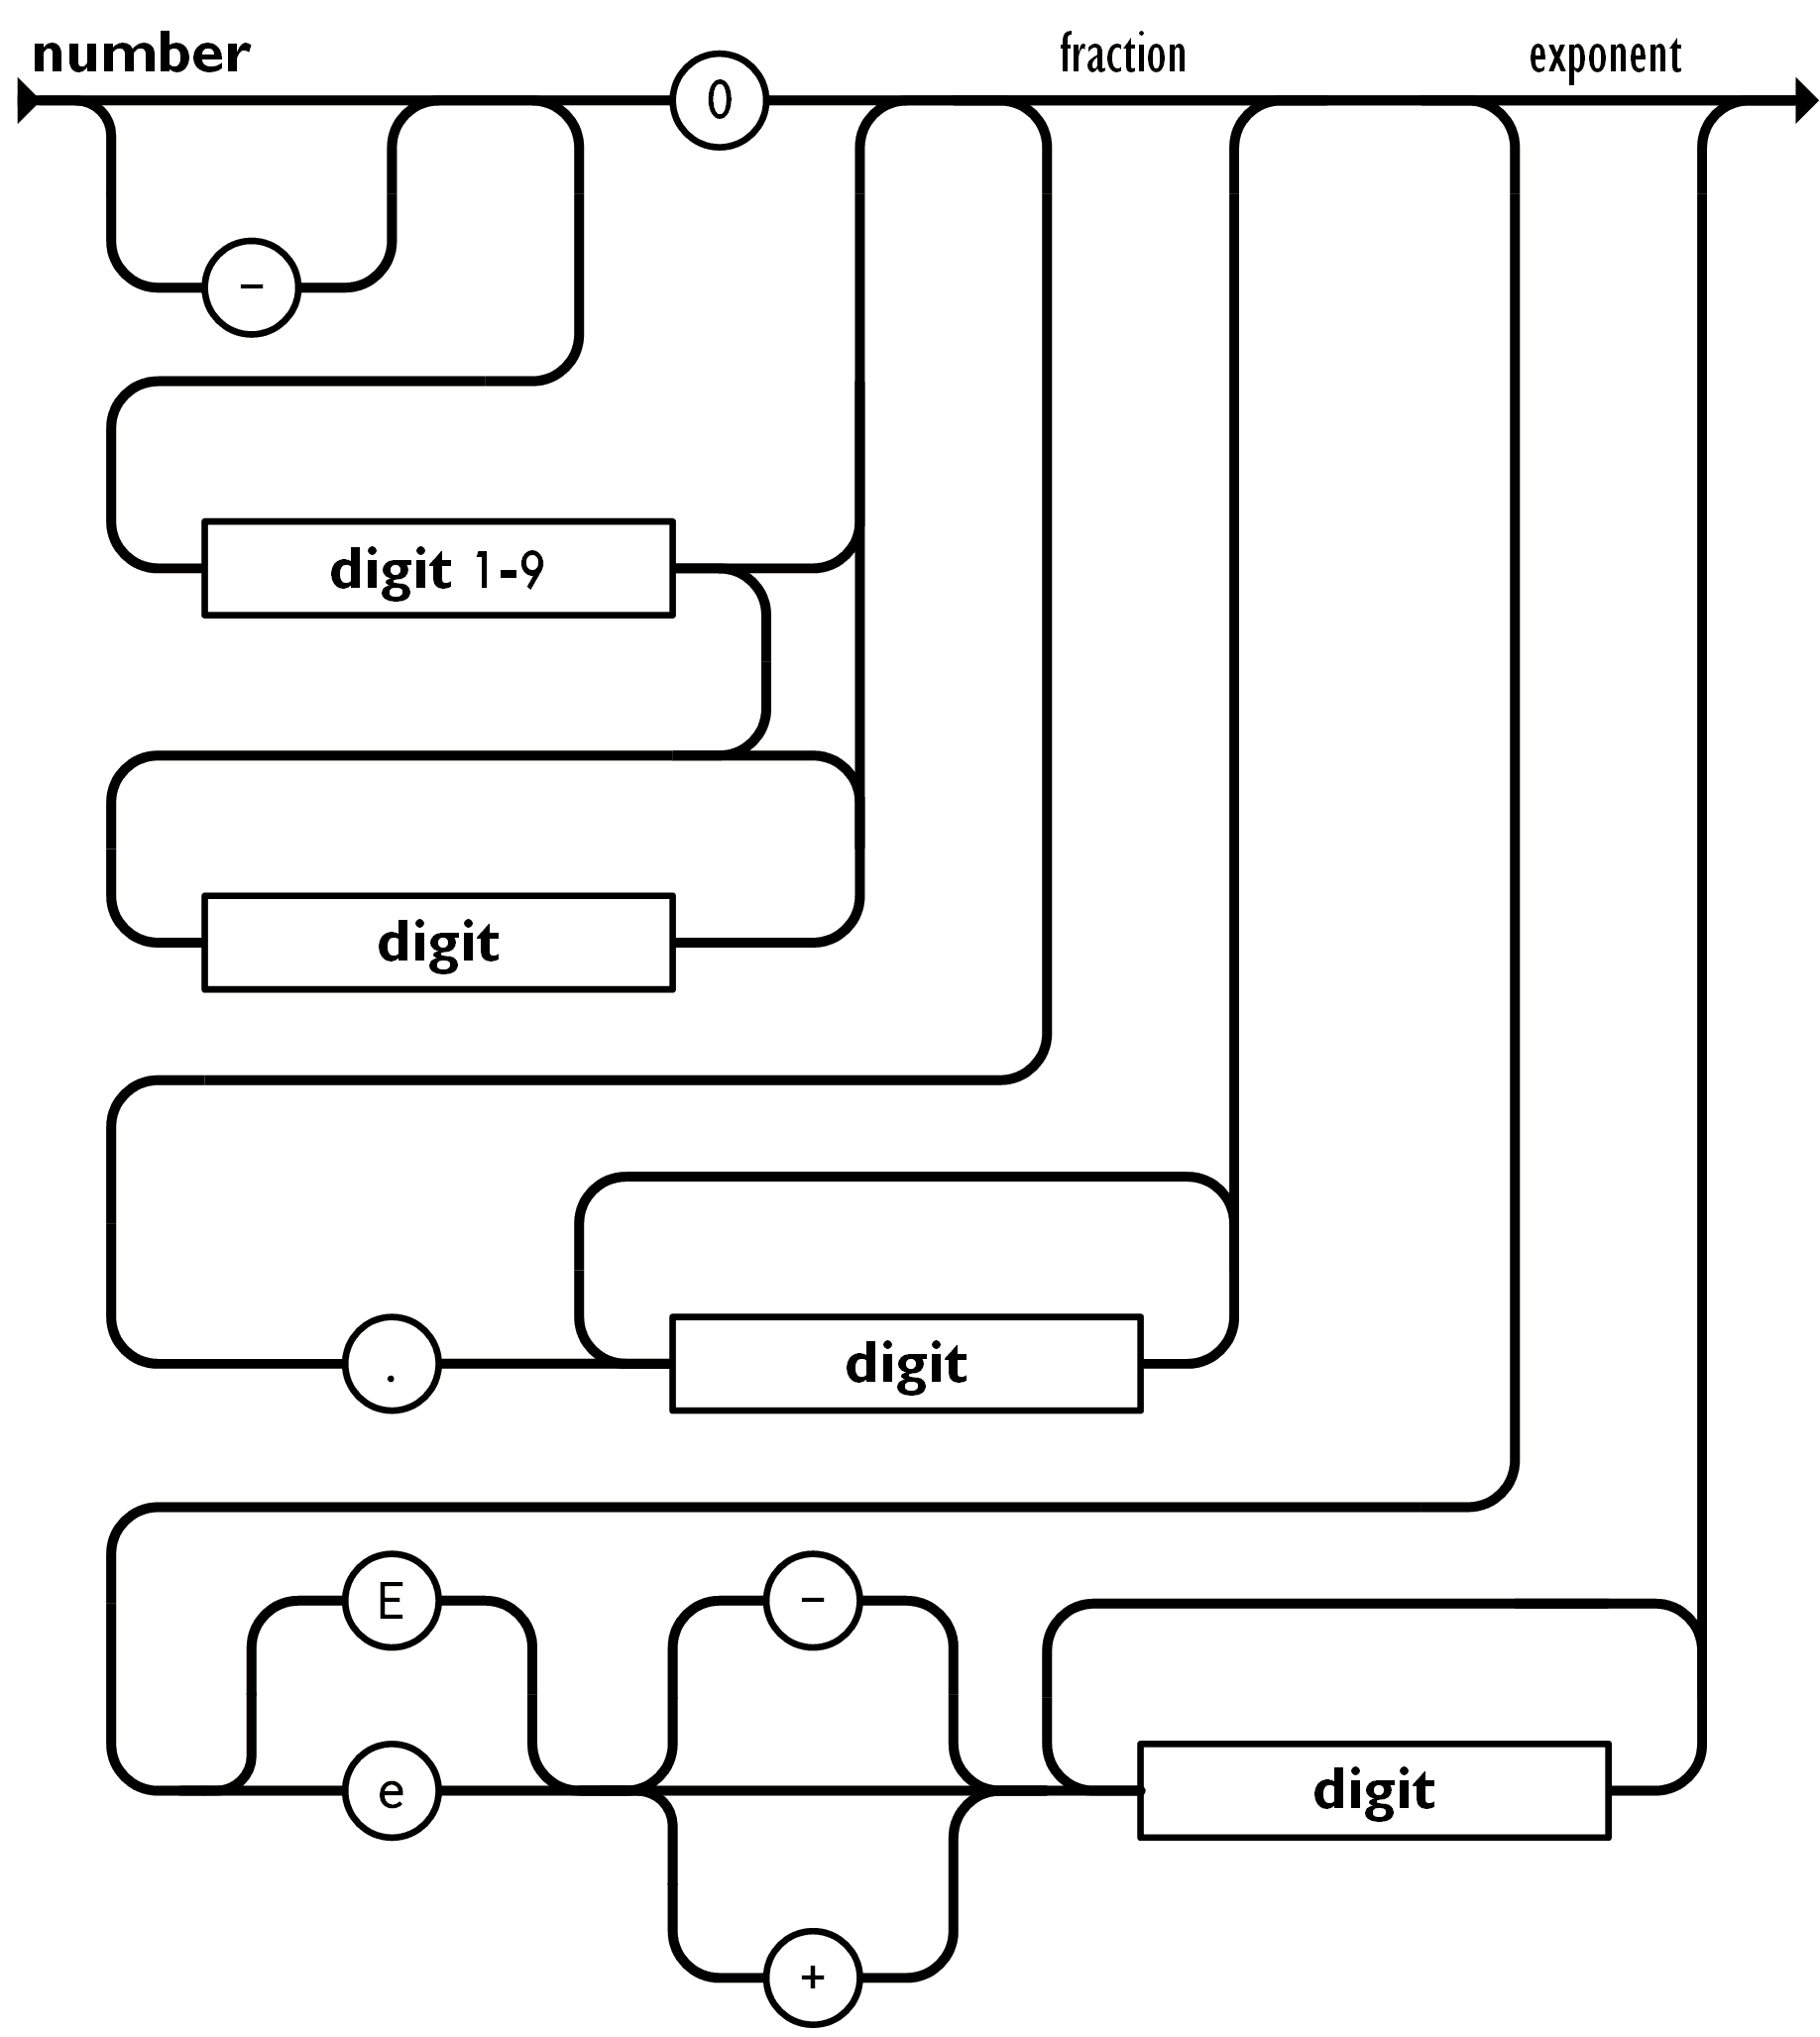
\includegraphics[scale=0.75]{jsonNumber}
    \caption[JSON Nummer]{De structuur van een JSON nummer.}
    \label{fig:jsonNumber}
\end{figure}

Tot slot zijn er de strings, deze representeren een tekst-waarde bestaande uit een sequentie van Unicode codepunten dewelke geïncapsuleerd zijn door aanhalingstekens die als Unicode code U+0022 hebben. Binnen deze aanhalingstekens zijn er echter enkele codepunten die niet gebruikt mogen worden, namelijk de karakters die moeten worden geëscaped. Dit zijn dan aanhalingstekens, backslash (U+005C), en de control karakters zijnde U+0000 tot en met U+OO1F
Voor sommige escape-reeksweergaven bestaande uit twee tekens bestaat er wel een representatie binnen de string.
Hieronder een representatie van zulke karakters.

\begin{itemize}
    \item \textbackslash “  aanhalingstekens
    \item \textbackslash \textbackslash \space backslash
    \item \textbackslash  / slash
    \item \textbackslash b backspace
    \item \textbackslash f form feed
    \item \textbackslash n nieuwe lijn
    \item \textbackslash r regelterugloopkarakter
    \item \textbackslash t karakter tabulatie karakter                 
\end{itemize}

Daarnaast kan ook elk codepunt weergegeven worden als een hexadecimale sequentie, de betekenis hiervan is vastgelegd in ISO/IEC 10646. Hexadecimale getallen kunnen zowel cijfers als kleine letters en hoofdletters van A tot F zijn, de cijfers zijn te vinden in Unicode van U+0030 tot en met U+0039. De hoofdletters zijn van U+0041 tot en met U+0046 terwijl de kleine letters te vinden zijn van U+0041 tot en met U+0046.
De codepunten die zich bevinden in het Basic Multilingual Plane, zijnde U+0000 tot en met U+FFFF, kunnen gerepresenteerd worden als een sequentie van zes karakters, namelijk een backslash gevolgd door een kleine letter u, en tot slot gevolgd door vier hexadecimale getallen die een codepunt encoderen.

\begin{figure}[h]
    \centering
    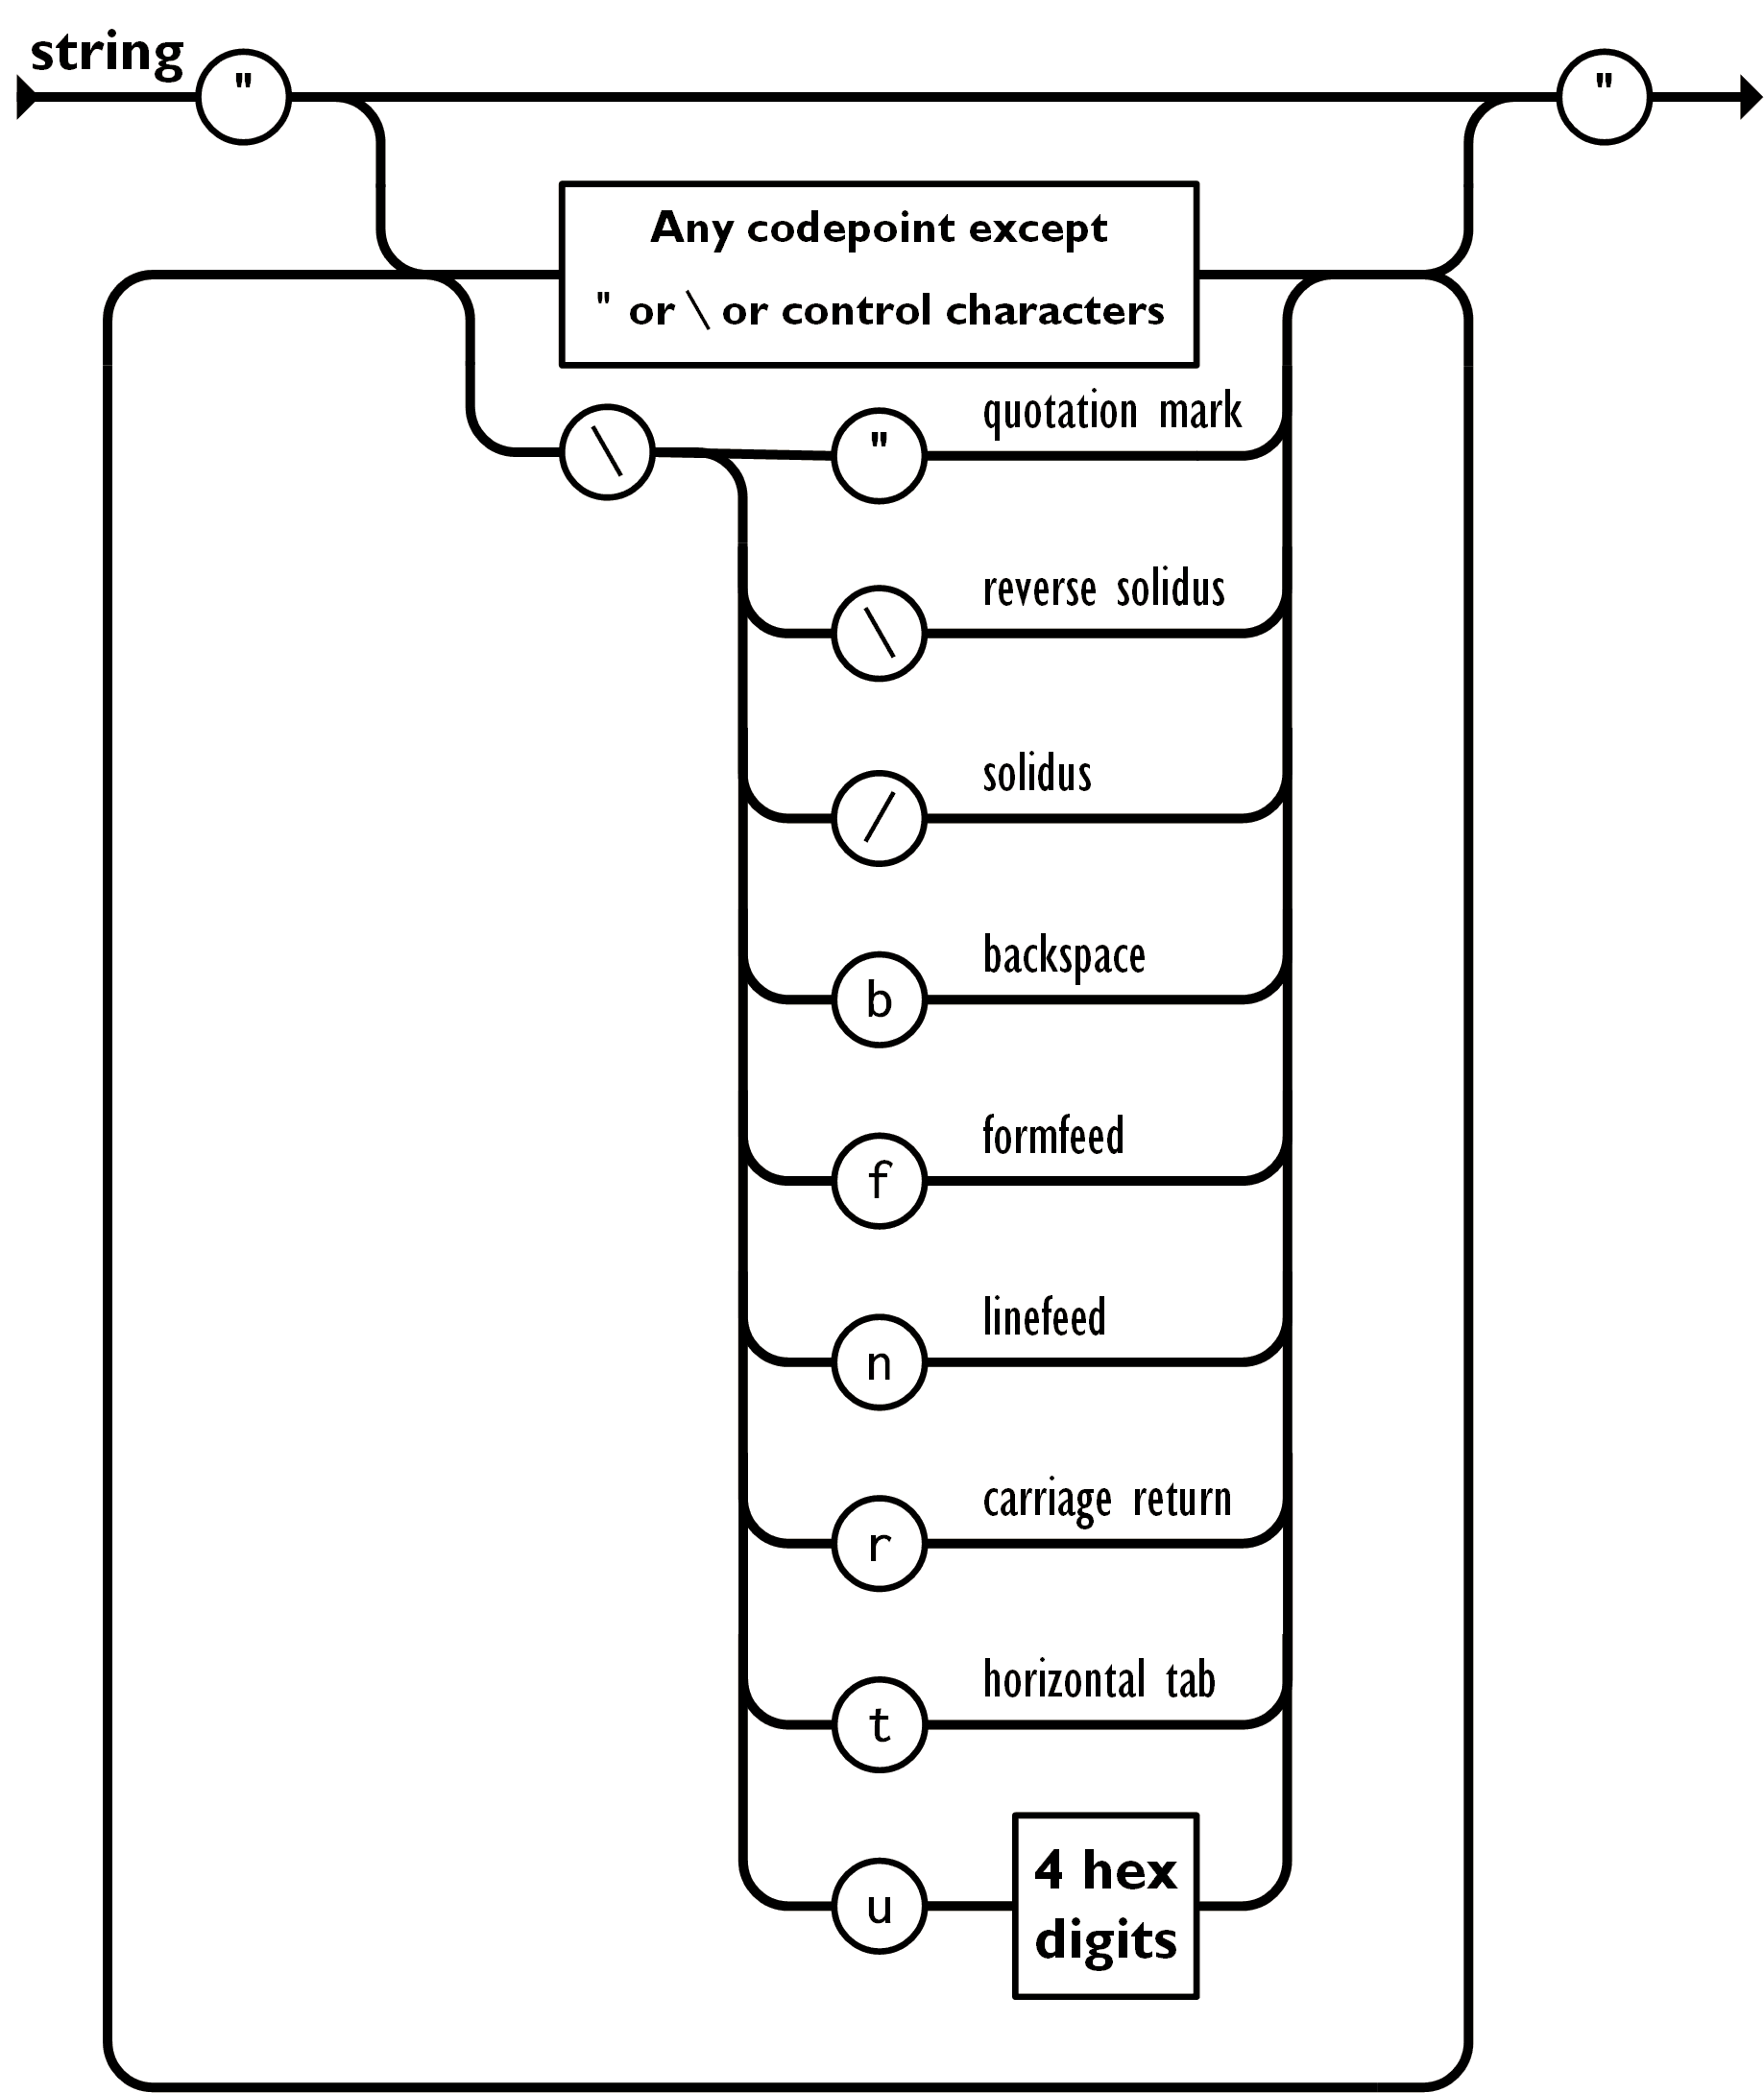
\includegraphics[scale=0.75]{jsonString}
    \caption[JSON String]{De structuur van een JSON string.}
    \label{fig:jsonString}
\end{figure}


\section{REST}
\label{sec:REST}

Representational State Transfer (REST) is zoals beschreven door \textcite{Fielding2000} een architecturale stijl voor het ontwerpen van gedistribueerde hypermediasystemen. Om een interface als RESTful te kunnen beschrijven moet deze voldoen aan zes principes dewelke hieronder zullen worden uitgelegd. 

\subsection{Client-Server}
\label{subsec:Client-Server}

Het eerste principe is Client-Server, hiermee wordt separation of concerns bedoeld. Door de concerns omtrent de user interface op te splitsen van de data storage concerns wordt de portabiliteit van de user interface verbeterd samen met de schaalbaarheid door het versimpelen van de server componenten. Als ook laat de opsplitsing toe dat de componenten zelfstandig kunnen groeien.
\subsection{Stateless}
\label{subsec:Stateless}

\subsection{Cacheable}
\label{subsec:Cacheable}

\subsection{Uniform interface}
\label{subsec:Uniform interface}

\subsection{Layered system}
\label{subsec:Layered system}

\subsection{Code on demand}
\label{subsec:Code on demand}

\subsection{Resources}
\label{subsec:Resources}
Daarnaast kan bij REST elk stuk informatie een resource zijn, dit kan van alles zijn zoals documenten, services, collecties van andere resources, afbeeldingen, en dergelijke. In sommige gevallen wordt “Everything as a resource”  een zevende principe van REST genoemd. 

Er valt af te leiden dat de definitie van een resource zeer abstract is, dit zorgt er voor dat cruciale features van de Web architectuur gebruikt kunnen worden. Eerst en vooral zorgt het voor generaliteit door meerdere bronnen en informatie te omvatten zonder deze te onderscheiden op basis van type of implementatie. Als volgt laat de abstracte definitie een late binding van de referentie aan een representatie toe, hierdoor kan content negotation plaatsvinden op basis van de kenmerken van de request. Tot slot maakt de abstracte definitie het mogelijk voor de auteur om een concept te refereren in plaats van een specifieke representatie van dat concept, hierdoor moeten links naar deze resource niet continue aangepast worden wanneer de representatie veranderd.
Deze links, ook wel Resource Identifiers genoemd, verwijzen naar een resource die gebruikt wordt in een interactie tussen componenten.

Om acties uit te voeren op een resource maakt REST gebruik van een representatie om de huidige of bedoelde staat van deze resource vast te leggen en deze uit te wisselen tussen componenten. Een representatie kan beschreven worden als een sequentie van bytes en bevat ook representatie metadata om deze bytes te beschrijven. Daarnaast bestaat een representatie uit verschillende onderdelen, namelijk de data, de metadata die de data beschrijft, en soms ook metadata die de metadata beschrijft, dit meestal met het doel om de integriteit van het bericht te verifiëren. Het dataformaat van een representatie is een media type ~\autocite{N.Freed1996}.




